\documentclass[aspectratio=169,11pt]{beamer}

% Theme and appearance
\usetheme{Madrid}
\usecolortheme{seahorse}
\usefonttheme{professionalfonts}

% Encoding (safe even on new LaTeX)
\usepackage[utf8]{inputenc}

% Packages
\usepackage{amsmath,amsthm,amssymb}
\usepackage{graphicx}
\usepackage{tikz}
\usetikzlibrary{calc}
\usepackage{pgfplots}
\pgfplotsset{compat=1.18}
\usepackage{algorithm,algorithmic}
\usepackage{booktabs}
\usepackage{multirow}
\usepackage{xcolor}
\usepackage{listings}
% \usepackage[caption=false]{subcaption} % <-- removed: incompatible with beamer
\usepackage{hyperref}

% Custom colors
\definecolor{navyblue}{RGB}{0,32,96}
\definecolor{crimson}{RGB}{178,34,52}
\definecolor{forest}{RGB}{34,139,34}
\definecolor{gold}{RGB}{255,215,0}
\definecolor{purple}{RGB}{128,0,128}

% Customize theme colors
\setbeamercolor{structure}{fg=navyblue}
\setbeamercolor{title}{fg=white,bg=navyblue}
\setbeamercolor{frametitle}{fg=white,bg=navyblue}
\setbeamercolor{section in toc}{fg=navyblue}

% Code listing settings
\lstset{
    language=Python,
    basicstyle=\ttfamily\small,
    keywordstyle=\color{navyblue}\bfseries,
    commentstyle=\color{forest}\itshape,
    stringstyle=\color{crimson},
    numbers=left,
    numberstyle=\tiny\color{gray},
    stepnumber=1,
    tabsize=2,
    showstringspaces=false,
    breaklines=true,
    frame=single,
    rulecolor=\color{gray!30}
}

% Title information
\title[Statistical Learning Theory]{Statistical Learning Theory}
\subtitle{Foundations for Data Science Applications}
\author[D. Ribeiro]{Diogo Ribeiro\\
\small ESMAD -- Escola Superior de Média Arte e Design\\
\small Lead Data Scientist, Mysense.ai}
\date{\today}

% Custom commands
\newcommand{\E}{\mathbb{E}}
\newcommand{\Var}{\operatorname{Var}}
\newcommand{\Cov}{\operatorname{Cov}}
\newcommand{\btheta}{\boldsymbol{\theta}}
\newcommand{\bx}{\mathbf{x}}
\newcommand{\by}{\mathbf{y}}
\newcommand{\bmu}{\boldsymbol{\mu}}
\newcommand{\bSigma}{\boldsymbol{\Sigma}}
\newcommand{\trace}{\operatorname{tr}}
\newcommand{\diag}{\operatorname{diag}}
\newcommand{\argmin}{\operatorname*{argmin}}
\newcommand{\argmax}{\operatorname*{argmax}}
\newcommand{\Real}{\mathbb{R}}
\newcommand{\Prob}{\mathbb{P}}

\begin{document}

% Title slide
\begin{frame}
\titlepage
\end{frame}

% Table of contents
\begin{frame}{Outline}
\tableofcontents
\end{frame}

\section{Introduction and Motivation}

\begin{frame}{From Statistics to Machine Learning}
\begin{columns}
\begin{column}[t]{0.6\textwidth}
\textbf{The Evolution of Learning from Data:}

\begin{itemize}
\item \textcolor{crimson}{Classical Statistics (1900-1970):}
  \begin{itemize}
  \item Fixed parametric models
  \item Hypothesis testing framework
  \item Small sample theory
  \item Focus on inference and explanation
  \end{itemize}
  
\item \textcolor{forest}{Machine Learning (1980-present):}
  \begin{itemize}
  \item Algorithmic approach
  \item High-dimensional data
  \item Prediction-focused
  \item Computational methods
  \end{itemize}
\end{itemize}
\end{column}
\begin{column}[t]{0.4\textwidth}
\begin{block}{Modern Data Science}
\begin{itemize}
\item Massive datasets
\item Complex patterns
\item Real-time decisions
\item Business impact
\end{itemize}
\end{block}

\begin{alertblock}{The Challenge}
How do we learn reliable patterns from finite data that generalize to unseen examples?
\end{alertblock}
\end{column}
\end{columns}
\end{frame}

\begin{frame}{Real-World Learning Problems}
\begin{table}
\centering
\small
\begin{tabular}{p{3cm}p{3.5cm}p{3cm}p{2cm}}
\toprule
\textbf{Application} & \textbf{Input ($X$)} & \textbf{Output ($Y$)} & \textbf{Goal} \\
\midrule
Netflix Recommendations & User history, ratings & Movie preferences & Predict ratings \\
\midrule
Medical Diagnosis & Symptoms, test results & Disease presence & Classification \\
\midrule
Financial Trading & Market data, news & Price movements & Forecast returns \\
\midrule
Fraud Detection & Transaction features & Fraud/legitimate & Binary classification \\
\midrule
Drug Discovery & Molecular structure & Biological activity & Regression \\
\bottomrule
\end{tabular}
\end{table}

\vspace{0.3cm}
\begin{block}{Common Pattern}
We observe training examples $(x_1, y_1), \ldots, (x_n, y_n)$ drawn from unknown distribution $P(X,Y)$ and want to predict $Y$ for new $X$.
\end{block}

\begin{alertblock}{Key Questions}
\begin{itemize}
\item How complex should our model be?
\item How confident can we be in predictions?
\item When will our model fail?
\end{itemize}
\end{alertblock}
\end{frame}

\begin{frame}{The Fundamental Learning Setup}
\begin{columns}
\begin{column}[t]{0.5\textwidth}
\textbf{Mathematical Framework:}

\begin{align}
\text{Input space:} \quad &\mathcal{X} \subseteq \Real^d\\
\text{Output space:} \quad &\mathcal{Y}\\
\text{Hypothesis class:} \quad &\mathcal{H} = \{h: \mathcal{X} \to \mathcal{Y}\}\\
\text{Loss function:} \quad &\ell: \mathcal{Y} \times \mathcal{Y} \to \Real^+
\end{align}

\textbf{Unknown joint distribution:} $(X, Y) \sim P(X,Y)$

\textbf{Training data:} $S = \{(x_i, y_i)\}_{i=1}^n$ i.i.d. from $P$
\end{column}
\begin{column}[t]{0.5\textwidth}
\textbf{Risk Functions:}

\begin{block}{Population Risk}
\[R(h) = \E_{(X,Y) \sim P}[\ell(h(X), Y)]\]
\textbf{True generalization error}
\end{block}

\begin{block}{Empirical Risk}
\[R_n(h) = \frac{1}{n}\sum_{i=1}^n \ell(h(x_i), y_i)\]
\textbf{Training error}
\end{block}

\begin{alertblock}{The Goal}
Find $h^* \in \argmin_{h \in \mathcal{H}} R(h)$ but we only observe $R_n(h)$
\end{alertblock}
\end{column}
\end{columns}
\end{frame}

\section{Mathematical Foundations}

\begin{frame}{Risk Decomposition: Understanding Prediction Error}
\textbf{Fundamental Decomposition:}

For any learning algorithm $\hat{h}$ trained on dataset $S$:

\begin{align}
R(\hat{h}) &= R(\hat{h}) - R(h^*_{\mathcal{H}}) + R(h^*_{\mathcal{H}}) - R^* + R^*\\
&= \underbrace{R(\hat{h}) - R(h^*_{\mathcal{H}})}_{\text{Estimation Error}} + \underbrace{R(h^*_{\mathcal{H}}) - R^*}_{\text{Approximation Error}} + \underbrace{R^*}_{\text{Bayes Risk}}
\end{align}

where:
\begin{itemize}
\item $R^* = \inf_{f} R(f)$ is the Bayes risk (irreducible error)
\item $h^*_{\mathcal{H}} = \argmin_{h \in \mathcal{H}} R(h)$ is the best function in our class
\end{itemize}

\begin{columns}
\begin{column}[t]{0.33\textwidth}
\begin{block}{Bayes Risk}
\textbf{Noise in data}
\begin{itemize}
\item Measurement error
\item Stochastic relationships
\item Missing variables
\end{itemize}
\end{block}
\end{column}
\begin{column}[t]{0.33\textwidth}
\begin{block}{Approximation Error}
\textbf{Model bias}
\begin{itemize}
\item Limited hypothesis class
\item Structural assumptions
\item Feature limitations
\end{itemize}
\end{block}
\end{column}
\begin{column}[t]{0.33\textwidth}
\begin{block}{Estimation Error}
\textbf{Finite sample effects}
\begin{itemize}
\item Random sampling
\item Optimization challenges
\item Model variance
\end{itemize}
\end{block}
\end{column}
\end{columns}
\end{frame}

\begin{frame}{Common Loss Functions}
\begin{columns}
\begin{column}[t]{0.5\textwidth}
\textbf{Regression Tasks:}

\begin{align}
\text{Squared Loss:} \quad &\ell(y, \hat{y}) = (y - \hat{y})^2\\
\text{Absolute Loss:} \quad &\ell(y, \hat{y}) = |y - \hat{y}|\\
\text{Huber Loss:} \quad &\ell_\delta(y, \hat{y}) = \begin{cases}
\frac{1}{2}(y - \hat{y})^2 & \text{if } |y - \hat{y}| \leq \delta \\
\delta|y - \hat{y}| - \frac{1}{2}\delta^2 & \text{otherwise}
\end{cases}
\end{align}

\textbf{Properties:}
\begin{itemize}
\item Squared: Differentiable, sensitive to outliers
\item Absolute: Robust, non-differentiable at 0
\item Huber: Best of both worlds
\end{itemize}
\end{column}
\begin{column}[t]{0.5\textwidth}
\textbf{Classification Tasks:}

\begin{align}
\text{0-1 Loss:} \quad &\ell(y, \hat{y}) = \mathbb{I}[y \neq \hat{y}]\\
\text{Hinge Loss:} \quad &\ell(y, \hat{y}) = \max(0, 1 - y\hat{y})\\
\text{Logistic Loss:} \quad &\ell(y, \hat{y}) = \log(1 + e^{-y\hat{y}})\\
\text{Cross-entropy:} \quad &\ell(y, \hat{y}) = -y\log(\hat{y}) - (1-y)\log(1-\hat{y})
\end{align}

\textbf{Trade-offs:}
\begin{itemize}
\item 0-1: What we care about, but non-convex
\item Hinge: Convex surrogate, sparse solutions
\item Logistic: Smooth, probabilistic interpretation
\end{itemize}
\end{column}
\end{columns}

\vspace{0.3cm}
\begin{alertblock}{Key Insight}
We often optimize surrogate losses (hinge, logistic) that are convex and differentiable, hoping they approximate the true loss (0-1) well.
\end{alertblock}
\end{frame}

\section{The Bias-Variance Tradeoff}

\begin{frame}{Bias-Variance Decomposition}
\textbf{Consider regression with squared loss.} For a fixed point $x$, decompose the expected squared error:

\begin{align}
\E[(\hat{f}(x) - y)^2] &= \E[(\hat{f}(x) - f(x) + f(x) - y)^2]\\
&= \E[(\hat{f}(x) - f(x))^2] + \E[(f(x) - y)^2] + 2\E[(\hat{f}(x) - f(x))(f(x) - y)]\\
&= \E[(\hat{f}(x) - f(x))^2] + \sigma^2 + 0
\end{align}

where $f(x) = \E[Y|X = x]$ and $\sigma^2 = \Var[Y|X = x]$.

\textbf{Further decomposition:}
\begin{align}
\E[(\hat{f}(x) - f(x))^2] &= \E[(\hat{f}(x) - \E[\hat{f}(x)] + \E[\hat{f}(x)] - f(x))^2]\\
&= \Var[\hat{f}(x)] + (\E[\hat{f}(x)] - f(x))^2\\
&= \text{Variance} + \text{Bias}^2
\end{align}

\begin{block}{Final Decomposition}
\[\boxed{\E[(\hat{f}(x) - y)^2] = \underbrace{\Var[\hat{f}(x)]}_{\text{Variance}} + \underbrace{(\E[\hat{f}(x)] - f(x))^2}_{\text{Bias}^2} + \underbrace{\sigma^2}_{\text{Noise}}}\]
\end{block}
\end{frame}

\begin{frame}{Understanding Bias and Variance}
\begin{columns}[t]
\begin{column}[t]{0.5\textwidth}
\begin{definition}[Bias]
\[\text{Bias}[\hat{f}(x)] = \E[\hat{f}(x)] - f(x)\]
\textbf{Systematic error} - how far off is our method on average?
\end{definition}

\begin{definition}[Variance]
\[\text{Variance}[\hat{f}(x)] = \E[(\hat{f}(x) - \E[\hat{f}(x)])^2]\]
\textbf{Random error} - how much does our method vary across datasets?
\end{definition}

\vspace{0.3cm}
\textbf{Intuition:}
\begin{itemize}
\item \textcolor{crimson}{High bias}: Model too simple, systematic underfitting
\item \textcolor{crimson}{High variance}: Model too complex, overfits to noise
\item \textcolor{forest}{Goal}: Find the sweet spot
\end{itemize}
\end{column}
\begin{column}[t]{0.5\textwidth}
\begin{figure}
\centering
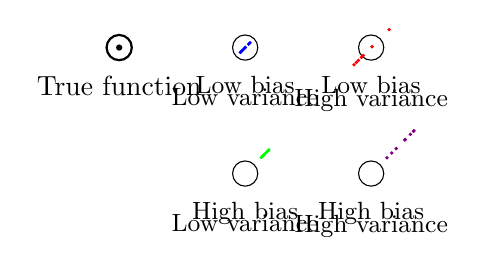
\begin{tikzpicture}[scale=0.8]
% Target
\draw[thick] (0,3) circle (0.2);
\fill (0,3) circle (0.05);
\node[below] at (0,2.7) {True function};

% Low bias, low variance
\draw (2,3) circle (0.2);
\foreach \i in {1,...,8}
  \fill[blue] ($(2,3) + 0.1*rand*(1,1)$) circle (0.03);
\node[below] at (2,2.7) {\small Low bias};
\node[below] at (2,2.5) {\small Low variance};

% Low bias, high variance
\draw (4,3) circle (0.2);
\foreach \i in {1,...,8}
  \fill[red] ($(4,3) + 0.3*rand*(1,1)$) circle (0.03);
\node[below] at (4,2.7) {\small Low bias};
\node[below] at (4,2.5) {\small High variance};

% High bias, low variance
\draw (2,1) circle (0.2);
\foreach \i in {1,...,8}
  \fill[green] ($(2.3,1.3) + 0.1*rand*(1,1)$) circle (0.03);
\node[below] at (2,0.7) {\small High bias};
\node[below] at (2,0.5) {\small Low variance};

% High bias, high variance
\draw (4,1) circle (0.2);
\foreach \i in {1,...,8}
  \fill[purple] ($(4.4,1.4) + 0.3*rand*(1,1)$) circle (0.03);
\node[below] at (4,0.7) {\small High bias};
\node[below] at (4,0.5) {\small High variance};
\end{tikzpicture}
\end{figure}

\begin{alertblock}{The Tradeoff}
Complex models: Low bias, high variance\\
Simple models: High bias, low variance
\end{alertblock}
\end{column}
\end{columns}
\end{frame}

\begin{frame}[fragile]{Interactive Demonstration: Polynomial Regression}
\textbf{Example:} Fitting polynomials of different degrees to a noisy sine wave

\begin{lstlisting}[basicstyle=\ttfamily\tiny]
import numpy as np
import matplotlib.pyplot as plt
from sklearn.preprocessing import PolynomialFeatures
from sklearn.linear_model import LinearRegression
from sklearn.pipeline import Pipeline

def true_function(x):
    return 1.5 * np.sin(2 * np.pi * x)

def generate_data(n_samples=50, noise_std=0.3):
    X = np.random.uniform(0, 1, n_samples)
    y = true_function(X) + np.random.normal(0, noise_std, n_samples)
    return X.reshape(-1, 1), y

# Generate multiple datasets for bias-variance analysis
n_datasets = 100
degrees = [1, 4, 15]
X_test = np.linspace(0, 1, 100).reshape(-1, 1)
y_test_true = true_function(X_test.ravel())

for degree in degrees:
    predictions = []
    for _ in range(n_datasets):
        X_train, y_train = generate_data()
        model = Pipeline([
            ('poly', PolynomialFeatures(degree)),
            ('linear', LinearRegression())
        ])
        model.fit(X_train, y_train)
        y_pred = model.predict(X_test)
        predictions.append(y_pred)
    
    predictions = np.array(predictions)
    bias_squared = np.mean((np.mean(predictions, axis=0) - y_test_true)**2)
    variance = np.mean(np.var(predictions, axis=0))
    print(f"Degree {degree}: Bias^2 = {bias_squared:.3f}, Variance = {variance:.3f}")
\end{lstlisting}
\end{frame}

\begin{frame}{Model Complexity and the U-Shaped Curve}
\begin{columns}
\begin{column}{0.5\textwidth}
\textbf{Training vs Test Error:}

\begin{figure}
\centering
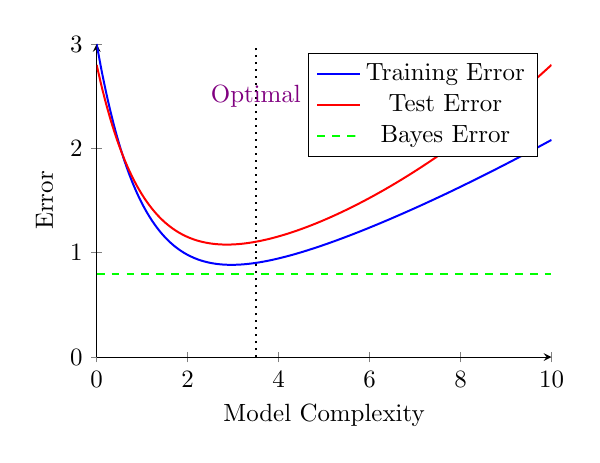
\begin{tikzpicture}[scale=0.9]
\begin{axis}[
    xlabel={Model Complexity},
    ylabel={Error},
    width=8cm,
    height=6cm,
    axis lines=left,
    xmin=0, xmax=10,
    ymin=0, ymax=3,
    legend pos=north east
]
\addplot[domain=0:10, samples=100, smooth, thick, blue] {0.5 + 2.5*exp(-x) + 0.05*x^1.5};
\addlegendentry{Training Error}
\addplot[domain=0:10, samples=100, smooth, thick, red] {0.8 + 2*exp(-x) + 0.02*x^2};
\addlegendentry{Test Error}
\addplot[domain=0:10, samples=100, smooth, thick, green, dashed] {0.8};
\addlegendentry{Bayes Error}
\draw[dotted, thick] (axis cs:3.5,0) -- (axis cs:3.5,3);
\node at (axis cs:3.5,2.5) {\textcolor{purple}{Optimal}};
\end{axis}
\end{tikzpicture}
\end{figure}
\end{column}
\begin{column}{0.5\textwidth}
\textbf{Key Observations:}

\begin{itemize}
\item \textcolor{forest}{Underfitting region}: Both training and test error are high
\item \textcolor{purple}{Sweet spot}: Test error is minimized
\item \textcolor{crimson}{Overfitting region}: Gap between training and test error grows
\end{itemize}

\vspace{0.3cm}
\begin{block}{Practical Implications}
\begin{itemize}
\item Use validation to find optimal complexity
\item Regularization helps control overfitting
\item More data allows more complex models
\item Early stopping prevents overfitting
\end{itemize}
\end{block}
\end{column}
\end{columns}

\vspace{0.3cm}
\begin{alertblock}{Modern Puzzle}
Deep learning models with millions of parameters often generalize well despite having more parameters than training examples.
\end{alertblock}
\end{frame}

\section{PAC Learning Theory}

% --- Entire PAC block must be inside a frame ---
\begin{frame}{PAC Learning Theory}
\begin{definition}[PAC Learnability]
A hypothesis class $\mathcal{H}$ is \textbf{PAC-learnable} if there exists an algorithm $A$ and polynomial function $p(\cdot, \cdot, \cdot, \cdot)$ such that:

For any distribution $D$ over $\mathcal{X}$, any target concept $c \in \mathcal{H}$, and any $\epsilon, \delta > 0$:

If $m \geq p(1/\epsilon, 1/\delta, \text{size}(c), \text{size}(\mathcal{X}))$, then
\[\Prob[\text{error}(A(S)) \leq \epsilon] \geq 1 - \delta\]

where $S$ is a training set of size $m$ drawn i.i.d. from $D$.
\end{definition}

\begin{columns}
\begin{column}{0.5\textwidth}
\textbf{Interpretation:}
\begin{itemize}
\item \textcolor{forest}{\textbf{Probably}}: With high probability $(1-\delta)$
\item \textcolor{forest}{\textbf{Approximately}}: Within $\epsilon$
\item \textcolor{forest}{\textbf{Correct}}: Low generalization error
\end{itemize}
\end{column}
\begin{column}[t]{0.5\textwidth}
\begin{block}{Sample Complexity}
The function $m(\epsilon, \delta)$ tells us how many examples we need to learn with accuracy $\epsilon$ and confidence $1-\delta$.
\end{block}

\begin{alertblock}{Key Question}
Which hypothesis classes are PAC-learnable and what's their sample complexity?
\end{alertblock}
\end{column}
\end{columns}
\end{frame}

\begin{frame}{VC Dimension: Measuring Hypothesis Class Complexity}
\begin{definition}[Shattering]
A set of points $\{x_1, \ldots, x_k\}$ is \textbf{shattered} by hypothesis class $\mathcal{H}$ if for every possible labeling $\{y_1, \ldots, y_k\} \in \{0,1\}^k$, there exists $h \in \mathcal{H}$ such that $h(x_i) = y_i$ for all $i$.
\end{definition}

\begin{definition}[VC Dimension]
The \textbf{VC dimension} of $\mathcal{H}$ is the size of the largest set that can be shattered by $\mathcal{H}$.
\[\text{VC}(\mathcal{H}) = \max\{k : \exists \text{ set of size } k \text{ that can be shattered by } \mathcal{H}\}\]
\end{definition}

\begin{columns}
\begin{column}{0.5\textwidth}
\textbf{Examples:}

\begin{itemize}
\item \textbf{Linear classifiers in $\Real^d$}: VC dim = $d + 1$
\item \textbf{Decision trees of depth $h$}: VC dim $\approx 2^h$
\item \textbf{Neural networks}: Complex, depends on architecture
\item \textbf{Nearest neighbor}: Infinite VC dimension
\end{itemize}
\end{column}
\begin{column}{0.5\textwidth}
\begin{figure}
\centering
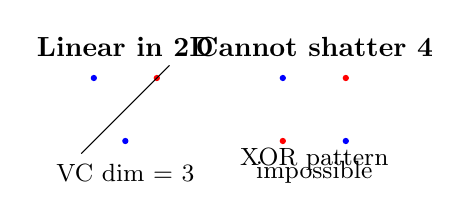
\begin{tikzpicture}[scale=0.8]
% Linear classifier in 2D - can shatter 3 points
\node at (1,3) {\textbf{Linear in 2D}};
\fill[blue] (0.5,2.5) circle (0.05);
\fill[red] (1.5,2.5) circle (0.05);
\fill[blue] (1,1.5) circle (0.05);
\draw (0.3,1.3) -- (1.7,2.7);
\node at (1,1) {\small VC dim = 3};

% Show that 4 points cannot always be shattered
\node at (4,3) {\textbf{Cannot shatter 4}};
\fill[blue] (3.5,2.5) circle (0.05);
\fill[red] (4.5,2.5) circle (0.05);
\fill[red] (3.5,1.5) circle (0.05);
\fill[blue] (4.5,1.5) circle (0.05);
\node at (4,1.2) {\small XOR pattern};
\node at (4,1) {\small impossible};
\end{tikzpicture}
\end{figure}
\end{column}
\end{columns}

\begin{theorem}[Fundamental Theorem of PAC Learning]
A hypothesis class $\mathcal{H}$ is PAC-learnable if and only if $\text{VC}(\mathcal{H}) < \infty$.
\end{theorem}
\end{frame}

\begin{frame}{Generalization Bounds}
\textbf{The power of VC theory:} Provides distribution-free generalization guarantees.

\begin{theorem}[VC Generalization Bound]
Let $\mathcal{H}$ be a hypothesis class with VC dimension $d$. Then with probability at least $1-\delta$, for all $h \in \mathcal{H}$:
\[R(h) \leq R_n(h) + \sqrt{\frac{8d\log(2n/d) + 8\log(4/\delta)}{n}}\]
\end{theorem}

\begin{columns}
\begin{column}{0.5\textwidth}
\textbf{Sample Complexity:}
For $(\epsilon, \delta)$-PAC learning:
\[m = O\left(\frac{d + \log(1/\delta)}{\epsilon^2}\right)\]

\textbf{Key insights:}
\begin{itemize}
\item Linear dependence on VC dimension
\item Quadratic dependence on accuracy $1/\epsilon$
\item Logarithmic dependence on confidence $1/\delta$
\item \textcolor{crimson}{Independent of data distribution!}
\end{itemize}
\end{column}
\begin{column}{0.5\textwidth}
\begin{block}{For Finite Hypothesis Classes}
If $|\mathcal{H}| = N < \infty$, then with probability $1-\delta$:
\[R(h) \leq R_n(h) + \sqrt{\frac{\log(N) + \log(1/\delta)}{2n}}\]
Sample complexity: $m = O\left(\frac{\log(N) + \log(1/\delta)}{\epsilon^2}\right)$
\end{block}

\begin{alertblock}{Trade-off}
Larger hypothesis classes (higher VC dimension) have:
\begin{itemize}
\item \textcolor{forest}{Lower approximation error}
\item \textcolor{crimson}{Higher estimation error}
\end{itemize}
\end{alertblock}
\end{column}
\end{columns}
\end{frame}

\section{Model Selection and Cross-Validation}

\begin{frame}{The Model Selection Challenge}
\textbf{Scenario:} We have multiple hypothesis classes $\mathcal{H}_1, \mathcal{H}_2, \ldots, \mathcal{H}_K$ and need to choose the best one.

\begin{columns}
\begin{column}{0.5\textwidth}
\textbf{Why is this hard?}
\begin{itemize}
\item Training error is optimistically biased
\item More complex models always fit training data better
\item Need unbiased estimate of generalization error
\item Limited data for evaluation
\end{itemize}

\vspace{0.3cm}
\textbf{Classical approach:}
\begin{itemize}
\item Information criteria (AIC, BIC)
\item Analytical penalties for complexity
\item Assumes specific model families
\end{itemize}
\end{column}
\begin{column}{0.5\textwidth}
\begin{block}{The Holdout Method}
\begin{enumerate}
\item Split data: Train (60\%) / Validation (20\%) / Test (20\%)
\item Train each model on training set
\item Evaluate on validation set
\item Select model with best validation performance
\item Report final performance on test set
\end{enumerate}
\end{block}

\begin{alertblock}{Problems with Holdout}
\begin{itemize}
\item Wastes data (especially problematic for small datasets)
\item High variance in estimates
\item Selection depends on particular split
\end{itemize}
\end{alertblock}
\end{column}
\end{columns}

\vspace{0.3cm}
\textbf{Solution:} Cross-validation - resampling approach that makes better use of data.
\end{frame}

\begin{frame}[fragile]{Cross-Validation: Theory and Practice}
\begin{columns}
\begin{column}[t]{0.55\textwidth}
\textbf{k-Fold Cross-Validation Algorithm:}

\begin{algorithm}[H]
\caption{k-Fold Cross-Validation}
\begin{algorithmic}[1]
\STATE Split data into $k$ roughly equal folds
\FOR{$i = 1$ to $k$}
\STATE Use fold $i$ as validation set
\STATE Use remaining $k-1$ folds as training set
\STATE Train model and compute validation error $e_i$
\ENDFOR
\STATE Return $\text{CV}_k = \frac{1}{k}\sum_{i=1}^k e_i$
\end{algorithmic}
\end{algorithm}

\textbf{Common choices:}
\begin{itemize}
\item $k = 5$ or $k = 10$ (good bias-variance tradeoff)
\item $k = n$ (Leave-One-Out CV, LOOCV)
\end{itemize}
\end{column}
\begin{column}[t]{0.45\textwidth}
\begin{lstlisting}[basicstyle=\ttfamily\tiny]
from sklearn.model_selection import cross_val_score
from sklearn.linear_model import Ridge
import numpy as np

# Generate sample data
from sklearn.datasets import make_regression
X, y = make_regression(n_samples=100, 
                       n_features=20, 
                       noise=0.1,
                       random_state=42)

# Test different regularization strengths
alphas = np.logspace(-4, 2, 20)
cv_scores = []

for alpha in alphas:
    model = Ridge(alpha=alpha)
    scores = cross_val_score(
        model, X, y, 
        cv=5, 
        scoring='neg_mean_squared_error'
    )
    cv_scores.append(-scores.mean())

# Select best alpha
best_alpha = alphas[np.argmin(cv_scores)]
print(f"Best alpha: {best_alpha:.4f}")
\end{lstlisting}
\end{column}
\end{columns}

\begin{block}{Statistical Properties of CV}
\begin{itemize}
\item \textbf{Bias}: $\text{Bias}[\text{CV}_k] \approx \frac{1}{k-1} \times \text{training set size effect}$
\item \textbf{Variance}: Decreases with $k$, but computational cost increases
\item \textbf{LOOCV}: Nearly unbiased but high variance, expensive for large $n$
\end{itemize}
\end{block}
\end{frame}

\begin{frame}{Advanced Cross-Validation Techniques}
\begin{columns}
\begin{column}{0.5\textwidth}
\textbf{Nested Cross-Validation:}
\begin{itemize}
\item Outer loop: Model assessment
\item Inner loop: Hyperparameter selection
\item Provides unbiased estimate of generalization
\item Essential for fair model comparison
\end{itemize}

\vspace{0.3cm}
\textbf{Stratified Cross-Validation:}
\begin{itemize}
\item Maintains class proportions in each fold
\item Important for imbalanced datasets
\item Reduces variance in estimates
\end{itemize}

\vspace{0.3cm}
\textbf{Time Series Cross-Validation:}
\begin{itemize}
\item Respects temporal ordering
\item Uses only past data for training
\item Expanding or sliding window approaches
\end{itemize}
\end{column}
\begin{column}{0.5\textwidth}
\begin{block}{Group Cross-Validation}
When data has natural clusters (e.g., patients, companies):
\begin{itemize}
\item Ensure same group doesn't appear in train and validation
\item Prevents data leakage
\item More conservative but realistic estimates
\end{itemize}
\end{block}

\begin{block}{Bootstrap Methods}
Alternative to CV:
\begin{itemize}
\item Sample with replacement
\item Out-of-bag samples for validation
\item Good for small datasets
\item Different bias-variance properties
\end{itemize}
\end{block}

\begin{alertblock}{Practical Tip}
For time series: Use \texttt{TimeSeriesSplit}\\
For groups: Use \texttt{GroupKFold}\\
For small data: Consider bootstrap\\
For hyperparameter tuning: Use nested CV
\end{alertblock}
\end{column}
\end{columns}
\end{frame}

\section{Applications and Case Studies}

\begin{frame}[fragile]{Case Study 1: Feature Selection for House Price Prediction}
\textbf{Problem:} Predict house prices with 80+ features, many potentially irrelevant.

\begin{lstlisting}[basicstyle=\ttfamily\tiny]
import pandas as pd
from sklearn.model_selection import validation_curve
from sklearn.feature_selection import SelectKBest, f_regression
from sklearn.linear_model import LinearRegression
from sklearn.pipeline import Pipeline
from sklearn.preprocessing import StandardScaler
from sklearn.datasets import load_boston

# Load data (Boston housing as example)
X, y = load_boston(return_X_y=True)

# Create pipeline with feature selection
pipe = Pipeline([
    ('scaler', StandardScaler()),
    ('selector', SelectKBest(f_regression)),
    ('regressor', LinearRegression())
])

# Test different numbers of features
param_range = range(1, X.shape[1] + 1)
train_scores, val_scores = validation_curve(
    pipe, X, y,
    param_name='selector__k',
    param_range=param_range,
    cv=5,
    scoring='neg_mean_squared_error'
)

# Plot bias-variance tradeoff
import matplotlib.pyplot as plt
train_mean = -train_scores.mean(axis=1)
val_mean = -val_scores.mean(axis=1)
val_std = val_scores.std(axis=1)

plt.figure(figsize=(10, 6))
plt.plot(param_range, train_mean, 'o-', label='Training MSE')
plt.plot(param_range, val_mean, 'o-', label='Validation MSE')
plt.fill_between(param_range, val_mean - val_std, val_mean + val_std, alpha=0.2)
plt.xlabel('Number of Features')
plt.ylabel('Mean Squared Error')
plt.legend()
plt.title('Feature Selection: Bias-Variance Tradeoff')
\end{lstlisting}
\end{frame}

\begin{frame}[fragile]{Case Study 2: Regularization in High-Dimensional Regression}
\textbf{Problem:} Gene expression data with 5{,}000 features and 100 samples.

\begin{lstlisting}[basicstyle=\ttfamily\tiny]
from sklearn.linear_model import Ridge, Lasso
from sklearn.model_selection import validation_curve
import numpy as np

# Simulate high-dimensional data
np.random.seed(42)
n_samples, n_features = 100, 5000
X = np.random.randn(n_samples, n_features)
true_coef = np.zeros(n_features)
true_coef[:10] = np.random.randn(10)  # Only first 10 are relevant
y = X @ true_coef + 0.1 * np.random.randn(n_samples)

# Compare Ridge and Lasso
alphas = np.logspace(-3, 2, 20)

ridge_train, ridge_val = validation_curve(
    Ridge(), X, y, param_name='alpha', param_range=alphas,
    cv=5, scoring='neg_mean_squared_error'
)

lasso_train, lasso_val = validation_curve(
    Lasso(max_iter=2000), X, y, param_name='alpha', param_range=alphas,
    cv=5, scoring='neg_mean_squared_error'
)

print("Ridge vs Lasso in high-dimensional setting:")
print("- Ridge: Continuous shrinkage, keeps all features")
print("- Lasso: Sparse solutions, automatic feature selection")
print("- Elastic Net: Combines both penalties")
\end{lstlisting}

\textbf{Key insights:} Lasso performs implicit feature selection, Ridge provides continuous shrinkage.
\end{frame}

\begin{frame}{Case Study 3: Model Selection in Practice}
\textbf{Problem:} Credit scoring with multiple algorithm choices.

\begin{table}
\centering
\small
\begin{tabular}{p{2.5cm}p{2cm}p{2cm}p{2cm}p{2cm}}
\toprule
\textbf{Model} & \textbf{CV Score} & \textbf{Std Error} & \textbf{Train Time} & \textbf{Interpretable?} \\
\midrule
Logistic Regression & 0.845 & 0.012 & 0.1s & Yes \\
Random Forest & 0.867 & 0.015 & 2.3s & Partial \\
Gradient Boosting & 0.874 & 0.011 & 45s & Partial \\
Neural Network & 0.871 & 0.018 & 15s & No \\
SVM (RBF) & 0.863 & 0.014 & 8s & No \\
\bottomrule
\end{tabular}
\end{table}

\begin{columns}
\begin{column}{0.5\textwidth}
\textbf{Statistical Considerations:}
\begin{itemize}
\item Is difference between 0.874 and 0.871 significant?
\item Paired t-test on CV folds
\item Practical vs statistical significance
\item Account for multiple comparisons
\end{itemize}
\end{column}
\begin{column}{0.5\textwidth}
\textbf{Business Considerations:}
\begin{itemize}
\item Interpretability requirements (regulation)
\item Prediction speed (real-time scoring)
\item Training cost (model updates)
\item Maintenance complexity
\end{itemize}
\end{column}
\end{columns}

\begin{alertblock}{Best Practice}
Don't always choose the model with highest CV score. Consider context: business requirements, operational constraints, and statistical significance.
\end{alertblock}
\end{frame}

\section{Modern Extensions and Future Directions}

\begin{frame}{Beyond Classical Theory: Modern Challenges}
\begin{columns}
\begin{column}{0.5\textwidth}
\textbf{The Double Descent Phenomenon:}
\begin{itemize}
\item Classical theory: U-shaped test error curve
\item Modern observation: Second descent in overparameterized regime
\item Challenges bias-variance decomposition
\item Common in deep learning
\end{itemize}

\vspace{0.3cm}
\textbf{High-Dimensional Statistics:}
\begin{itemize}
\item $p \gg n$ scenarios (genomics, finance)
\item Curse of dimensionality
\item Blessing of dimensionality (concentration)
\item Sparsity assumptions crucial
\end{itemize}
\end{column}
\begin{column}{0.5\textwidth}
\begin{figure}
\centering
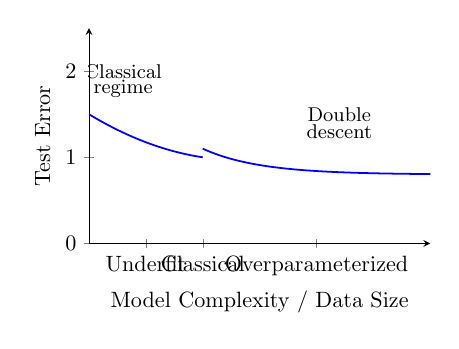
\begin{tikzpicture}[scale=0.8]
\begin{axis}[
    xlabel={Model Complexity / Data Size},
    ylabel={Test Error},
    width=7cm,
    height=5cm,
    axis lines=left,
    xmin=0, xmax=3,
    ymin=0, ymax=2.5,
    xtick={0.5, 1, 2},
    xticklabels={Underfit, Classical, Overparameterized}
]
\addplot[domain=0:1, samples=50, smooth, thick, blue] {1.5 - 0.8*x + 0.3*x^2};
\addplot[domain=1:3, samples=50, smooth, thick, blue] {0.8 + 0.3*exp(-(x-1)*2)};
\node at (axis cs:0.3,2) {\small Classical};
\node at (axis cs:0.3,1.8) {\small regime};
\node at (axis cs:2.2,1.5) {\small Double};
\node at (axis cs:2.2,1.3) {\small descent};
\end{axis}
\end{tikzpicture}
\end{figure}

\begin{block}{Modern Theory Needs}
\begin{itemize}
\item Implicit regularization in SGD
\item Benign overfitting conditions
\item Role of initialization and architecture
\item Distribution-dependent bounds
\end{itemize}
\end{block}
\end{column}
\end{columns}

\begin{alertblock}{Open Questions}
Why do overparameterized models generalize well? How should we modify classical learning theory for the modern era?
\end{alertblock}
\end{frame}

\begin{frame}{Emerging Frontiers in Learning Theory}
\begin{columns}
\begin{column}{0.5\textwidth}
\textbf{Causal Learning:}
\begin{itemize}
\item Beyond correlation to causation
\item Structural causal models
\item Invariant risk minimization
\item Domain adaptation and robustness
\end{itemize}

\vspace{0.3cm}
\textbf{Meta-Learning:}
\begin{itemize}
\item Learning to learn across tasks
\item Few-shot learning
\item Model-agnostic meta-learning (MAML)
\item Bayesian optimization for hyperparameters
\end{itemize}

\vspace{0.3cm}
\textbf{Continual Learning:}
\begin{itemize}
\item Learning without forgetting
\item Catastrophic forgetting problem
\item Elastic weight consolidation
\item Progressive networks
\end{itemize}
\end{column}
\begin{column}{0.5\textwidth}
\textbf{Federated Learning:}
\begin{itemize}
\item Distributed learning with privacy
\item Communication constraints
\item Non-IID data distributions
\item Differential privacy guarantees
\end{itemize}

\vspace{0.3cm}
\textbf{Robust Learning:}
\begin{itemize}
\item Adversarial examples
\item Distribution shift
\item Worst-case guarantees
\item Certified defenses
\end{itemize}

\vspace{0.3cm}
\begin{block}{Practical Implications}
Modern ML applications require:
\begin{itemize}
\item Robustness to distribution shift
\item Privacy-preserving algorithms
\item Continual adaptation
\item Causal understanding
\end{itemize}
\end{block}
\end{column}
\end{columns}

\textbf{The Future:} Integration of classical statistical learning with modern ML challenges.
\end{frame}

\section{Summary and Conclusions}

\begin{frame}{Key Takeaways}
\begin{columns}
\begin{column}{0.5\textwidth}
\textbf{Fundamental Concepts:}
\begin{itemize}
\item \textcolor{forest}{Risk decomposition}: Understand sources of error
\item \textcolor{forest}{Bias-variance tradeoff}: Balance simplicity and complexity
\item \textcolor{forest}{PAC learning}: Formal guarantees for learnability
\item \textcolor{forest}{VC dimension}: Measure of hypothesis class complexity
\item \textcolor{forest}{Cross-validation}: Practical model selection tool
\end{itemize}

\vspace{0.3cm}
\textbf{Practical Guidelines:}
\begin{itemize}
\item Start with simple baselines
\item Use proper validation methodology
\item Consider business constraints
\item Understand your data and domain
\item Monitor for distribution shift
\end{itemize}
\end{column}
\begin{column}{0.5\textwidth}
\textbf{Modern Challenges:}
\begin{itemize}
\item High-dimensional data requires new techniques
\item Deep learning challenges classical theory
\item Robustness and fairness are crucial
\item Causality matters for decision-making
\end{itemize}

\vspace{0.3cm}
\begin{block}{The Big Picture}
Statistical learning theory provides:
\begin{itemize}
\item Principled foundation for ML
\item Tools for understanding when/why methods work
\item Guidance for method selection
\item Framework for developing new algorithms
\end{itemize}
\end{block}

\begin{alertblock}{Remember}
Theory guides practice, but practical considerations (interpretability, speed, fairness) often dominate real decisions.
\end{alertblock}
\end{column}
\end{columns}
\end{frame}

\begin{frame}{Next Steps in the Data Science Track}
\begin{columns}
\begin{column}{0.5\textwidth}
\textbf{Immediate Next Topics:}
\begin{enumerate}
\item \textbf{Feature Engineering \& Selection}
   \begin{itemize}
   \item Automated feature engineering
   \item Dimensionality reduction
   \item Feature importance methods
   \end{itemize}

\item \textbf{Causal Inference}
   \begin{itemize}
   \item From correlation to causation
   \item Experimental design
   \item Observational causal methods
   \end{itemize}

\item \textbf{Model Interpretability}
   \begin{itemize}
   \item SHAP, LIME, and friends
   \item Global vs local explanations
   \item Interpretable model classes
   \end{itemize}
\end{enumerate}
\end{column}
\begin{column}{0.5\textwidth}
\textbf{Hands-on Projects:}
\begin{itemize}
\item Implement bias-variance decomposition from scratch
\item Build cross-validation framework
\item Apply theory to real dataset
\item Compare multiple algorithms systematically
\end{itemize}

\vspace{0.3cm}
\textbf{Further Reading:}
\begin{itemize}
\item Hastie, Tibshirani, Friedman: \emph{Elements of Statistical Learning}
\item Shalev-Shwartz, Ben-David: \emph{Understanding Machine Learning}
\item Vapnik: \emph{The Nature of Statistical Learning Theory}
\end{itemize}
\end{column}
\end{columns}

\vspace{0.5cm}
\begin{center}
\textcolor{navyblue}{\Large \textbf{Statistical learning theory is the foundation that makes all of data science principled and reliable.}}
\end{center}
\end{frame}

\begin{frame}
\begin{center}
{\Huge Thank You}

\vspace{0.8cm}

\textbf{Questions \& Discussion}

\vspace{1cm}

\textbf{Diogo Ribeiro}\\
ESMAD -- Escola Superior de Média Arte e Design\\
Lead Data Scientist, Mysense.ai\\

\vspace{0.5cm}

\texttt{dfr@esmad.ipp.pt}\\
\texttt{https://orcid.org/0009-0001-2022-7072}

\vspace{0.8cm}

\textit{Slides and code available at:}\\
\texttt{github.com/diogoribeiro7/academic-presentations}

\vspace{0.5cm}

\textit{Next: Feature Engineering \& Selection}
\end{center}
\end{frame}

\end{document}
